Date : 8 december 2023

\subsubsection{Moduleren}
Het aanbrengen van informatie in een draaggolf wordt vaak gemodelleerd als:

\[ U_c(t) = \hat{U}_c \cdot \cos(2\pi f_c t + \alpha) \]

waarbij:
\begin{itemize}
  \item \(U_c(t)\) de gemoduleerde draaggolf is,
  \item \(\hat{U}_c\) de amplitude van de draaggolf,
  \item \(f_c\) de frequentie van de draaggolf,
  \item \(\alpha\) de fasehoek.
\end{itemize}

Amplitude Modulatie (AM) houdt in dat de amplitude \(\hat{U}_c\) wordt gevarieerd.

Frequentiemodulatie (FM) houdt in dat de frequentie \(f_c\) wordt gevarieerd.

Phasemodulatie (PM) houdt in dat de fasehoek \(\alpha\) wordt gevarieerd.

\begin{figure}[H]
\centering
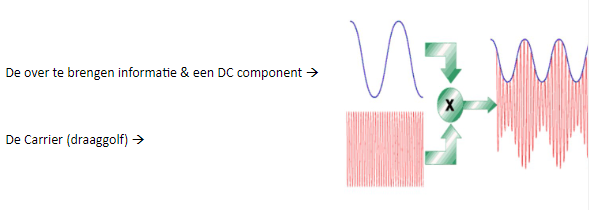
\includegraphics[scale=0.8]{AM.png}
\caption{Amplitude Modulatie}
\end{figure}

Modulatiediepte (\(m\)) geeft aan hoe sterk er gemoduleerd wordt en wordt bepaald door:

\[ m = \frac{\hat{U}_m}{\hat{U}_c} \times 100\% \]

waarbij:
\begin{itemize}
  \item \(m\) de modulatiediepte is,
  \item \(\hat{U}_m\) de amplitude van het informatiesignaal is,
  \item \(\hat{U}_c\) de amplitude van het carriersignaal is.
\end{itemize}

In het frequentiespectrum ontstaan drie frequentiecomponenten (wanneer het informatiesignaal uit slechts één frequentie bestaat):

\begin{enumerate}
  \item De carrierfrequentie \(f_c\)
  \item Zijband 1: \(f_c + f_m\)
  \item Zijband 2: \(f_c - f_m\)
\end{enumerate}

waarbij:
\begin{itemize}
  \item \(f_c\) de draaggolf frequentie is,
  \item \(f_m\) de frequentie van het informatiesignaal is.
\end{itemize}

\begin{figure}[H]
\centering
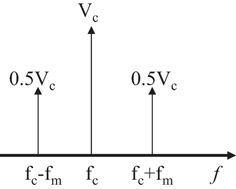
\includegraphics[scale=0.8]{frequentiespectrum AM.png}
\caption{Frequent AM}
\end{figure}

Het vermogensspectrum is als volgt te bepalen:

\begin{itemize}
  \item Voor de Carrier geldt:
  \[ P_c = \left(\frac{\hat{U}_c}{\sqrt{2}}\right)^2 \div R_{\text{load}} \, \text{(Watt)} \]

  \item Voor elke van de zijbanden geldt:
  \[ P_{zb} = \left(\frac{m\hat{U}_c}{2\sqrt{2}}\right)^2 \div R_{\text{load}} = \frac{m^2}{4} \cdot \left(\frac{\hat{U}_c}{\sqrt{2}}\right)^2 = \frac{P_c \cdot m^2}{4} \]
\end{itemize}

waarbij:
\begin{itemize}
  \item \(P_c\) het vermogen van de carrier is,
  \item \(P_{zb}\) het vermogen van elke zijband is,
  \item \(\hat{U}_c\) de amplitude van het carriersignaal is,
  \item \(m\) de modulatiediepte is,
  \item \(R_{\text{load}}\) de belastingsweerstand is.
\end{itemize}

\vspace{0.5cm}
Wat zijn de voordelen van AM?
\begin{itemize}
  \item Eenvoudige demodulatie.
  \item De carrier is altijd aanwezig en afstembaar.
\end{itemize}

Wat zijn de nadelen van AM?
\begin{itemize}
  \item Storingsgevoeligheid (amplitude).
  \item Relatief veel vermogen waarin geen informatie zit.
\end{itemize}

\subsubsection{Single Side Band (SSB)}
Single Side Band (SSB) is een modulatietechniek die wordt gebruikt in communicatiesystemen. In SSB wordt slechts één zijband van het gemoduleerde signaal overgedragen, samen met de draaggolf, in plaats van beide zijbanden zoals bij Amplitude Modulatie (AM).

De wiskundige representatie van een SSB-signaal is als volgt:

\[ U(t) = A_c \cdot m(t) \cdot \cos(2\pi f_c t) \]

waarbij:
\begin{itemize}
  \item \(U(t)\) is het SSB-signaal,
  \item \(A_c\) is de amplitude van de draaggolf,
  \item \(m(t)\) is het informatiesignaal,
  \item \(f_c\) is de frequentie van de draaggolf.
\end{itemize}

\begin{figure}[H]
\centering
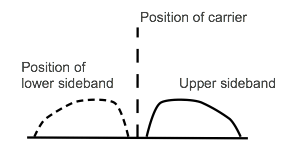
\includegraphics[scale=0.8]{single-sideband-ssb-overview.png}
\caption{single side band overview}
\end{figure}

De voordelen van SSB zijn onder andere een efficiënter gebruik van het radiospectrum en verminderde vermogensvereisten. Echter, demodulatie van SSB vereist complexere apparatuur in vergelijking met AM.

\subsubsection{Frequentie Modulatie (FM)}
FM is een goed alternatief voor AM.

Voordelen:
\begin{itemize}
  \item Minder storingsgevoelig, informatie zit niet in de amplitude.
  \item Constant vermogen.
\end{itemize}

Nadelen:
\begin{itemize}
  \item Grotere bandbreedte.
  \item Complexere hardware.
\end{itemize}

\begin{figure}[H]
\centering
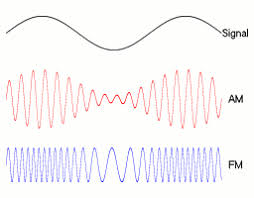
\includegraphics[scale=0.8]{FM.jpeg}
\caption{FM vs AM}
\end{figure}
    